\documentclass[a4paper,14pt]{extreport}
\usepackage[utf8]{inputenc}
\usepackage[T1]{fontenc}
%\usepackage{lmodern}
\usepackage[english, russian]{babel}
\usepackage{indentfirst}
\usepackage{amssymb,amsfonts,amsmath,mathtext,cite,enumerate,float}
\usepackage[dvips]{graphicx}
\usepackage{titlesec}

\usepackage{geometry}
\usepackage{enumitem}
\geometry{left=2cm}
\geometry{right=2cm}
\geometry{top=0.5cm}
\geometry{bottom=2cm}

\titleformat{\chapter}[block]{\normalfont\bfseries}{\thechapter}{20pt}{}{}
%\addto\captionsrussian{\renewcommand{\chaptername}{}}
%\renewcommand{\thechapter}{}

\graphicspath{{../introduction/images/},{./images/}}

% Title Page
\title{Введение в дипломную работу}
\author{Елисеев Владислав}

\makeatletter
\bibliographystyle{unsrt}
\renewcommand{\@biblabel}[1]{#1.} 
\makeatother
\parindent=1cm

\sloppy
\hyphenation{STan-ford}

\newenvironment{compactlist}{
    \begin{list}
    {{$\bullet$}}
    {
        \setlength\partopsep{0pt}
        \setlength\parskip{0pt}
        \setlength\parsep{0pt}
        \setlength\topsep{0pt}
        \setlength\itemsep{0pt}                        
    }
}{
    \end{list}
}

\begin{document}
\begin{titlepage}

\begin{center}


\includegraphics[width=0.3\linewidth]{msu_title}

{\small
МОСКОВСКИЙ ГОСУДАРСТВЕННЫЙ УНИВЕРСИТЕТ имени М.В.~ЛОМОНОСОВА \\
ФАКУЛЬТЕТ ВЫЧИСЛИТЕЛЬНОЙ МАТЕМАТИКИ И КИБЕРНЕТИКИ \\
КАФЕДРА СИСТЕМНОГО ПРОГРАММИРОВАНИЯ
}
\end{center}

\vfill
\vfill
\begin{center}
\Large{\textbf{Отчет по дипломной работе}} \\
~\\
\Large{Генерация моделей на унифицированном языке моделирования по описаниям предметных областей и~задач планирования}
\end{center}
\vfill
\vfill
\vfill
\vfill
\begin{flushright}
Исполнитель: \\
студент 527 группы Елисеев Владислав
\end{flushright}
\vfill
\begin{flushright}
Научный руководитель: \\
к.ф.-м.н. Малышко Виктор Васильевич
\end{flushright}
  
\vfill
\vfill
\vfill
\vfill
\begin{center}
  Москва\\
  2013
\end{center}  
\end{titlepage}


\newgeometry{top=2cm, bottom=2cm, left=2cm, right=2cm}

\setcounter{page}{1}
\linespread{1}
\normalsize

\section*{Введение}
	Одна из задач в области искусственного интеллекта~--- задача планирования. Планированием называется процесс выработки последовательности действий, позволяющей достичь цели \cite{norwig-ai}. Задача планирования часто встает у агентов, которым нужно найти последовательность действий, выполнив которые он достигнет некоторой своей цели. Агентом можно назвать все, что воспринимает свою среду с помощью некоторых датчиков и воздействует на нее с помощью некоторых механизмов. Примерами использования планирования может служить следующее: планирование управлением механическими приводами робота-мусоросборника, планирование распределения транспортных средств для перевозок различных видов топлива и сырья на нефтеперерабатывающем заводе. 

	Контекст задачи планирования, модель мира, в котором возникает задача,  называется предметной областью.  
	
	В 1971 году для представления знаний о предметных областях был разработан формальный текстовый язык STRIPS \cite{strips} (STanford Research Institute Problem Solver). В этом языке выделяются три основных понятия~--- \textit{состояние среды} (мира), \textit{действие} (механизмы воздействия на среду), \textit{цель} (целевое состояние мира). Состояния задаются в виде некоторого набора фактов об объектах и отношениях между ними, которые считаются истинными в этом состоянии. Действия задаются с использованием набора ограничений на состояние (предусловие), и набора положительных и отрицательных фактов (эффекты). \textit{Предусловие} должно выполняться для того, чтобы применение действия было допустимым в данном состоянии. \textit{Эффект} задает то, как меняется состояние при применении действия~--- положительные факты добавляются к состоянию, отрицательные~--- удаляются. \textit{Цель}, или целевое состояние, задается как набор ограничений, которые должны быть удовлетворены в данном состоянии. Также в STRIPS вводится гипотеза замкнутости мира (CWA, \textit{Closed World Assumption}), которая означает, что факты, не перечисленные в описании состояния, считаются ложными.
	
	В 1987 году был предложен язык ADL (Action Description Language, язык описания действий) похожий на STRIPS, но включающий в себя еще несколько особенностей, из которых можно отметить следующие:
	\begin{compactlist}
	    \item предположение об открытом мире - факты, не перечисленные в состоянии, считаются неизвестными;
	    \item возможность использования кванторов и дизъюнктов для задания цели;
	    \item возможность использования условных эффектов;
	    \item наличие встроенного предиката равенства для сравнения объектов;
	    \item возможность типизации переменных;
	    \item и т.д.
	\end{compactlist}
    
    В 1988 году появился язык PDDL\cite{pddl3} (Planning Domain Definition Language, язык описания предметных областей и задач планирования) как попытка стандартизации существующих на тот момент языков описания предметных областей и задач планирования. Также это сделало возможным создание IPC~--- International Planing Competition~--- международных соревнований по созданию планировщиков. На данный момент PDDL стал стандартом де-факто для описания знаний систем планирования.
  
    В настоящее время большую популярность приобретают графические представления, основанные на объектных спецификациях. В нашем случае, графическое представление знаний может быть более удобным для использования людьми, нежели текстовое представление. Для графического моделирования и удовлетворения нужд программной индустрии был разработан язык UML\cite{rambo-uml2} (Unified Modeling Language, унифицированный язык моделирования), но его возможности оказались шире, поэтому он используется и в других областях. Например, его можно использовать для представления знаний систем планирования в виде UML-моделей. Для задания дополнительных ограничений на UML-модели может быть использован язык OCL\cite{ocl}. Для создания UML-моделей существует множество редакторов, что делает возможность задания знаний среды и задачи планирования в графическом представлении более привлекательной. 
    
    Применение объектных спецификаций для задания знаний систем планирования является актуальной темой для исследований.  По этой теме на международной конференции ICAPS (International Conference on Automated Planning and Scheduling) было представлено несколько докладов \cite{icaps-1, icaps-2}.
    
   
    
\section*{Постановка задачи}

     Из-за наличия разных представлений одних и тех же знаний наряду с проблемой соответствия этих представлений друг другу встает задача преобразования одних представлений в другие. 

    В данной дипломной работе предполагается создать программное средство, которое будет автоматизировать преобразование представлений знаний систем планирования из текстового (PDDL-представления) в графическое (в виде UML-моделей). Получение UML-представления может быть полезно, так как:
    \begin{itemize}
        \item UML-модели более наглядны, составлять UML базы знаний могут эксперты, не знакомые с PDDL;
        \item UML-модель может быть отредактирована в UML-редакторе, и при необходимости её можно транслировать в другие языки (Java, PDDL, и~ др.);
        \item существуют средства валидации и исполнения UML-моделей для проверки корректности знаний\cite{use}; 
        \item существуют средства трансформации моделей, с помощью которых можно из UML-модели предметной области получить описания задач для этой предметной области.
    \end{itemize}


   \par  Пусть $K$~--- знания системы планирования, $K = \langle D, T \rangle$, где $D$~--- знания о предметной области, $T = \{t_1, t_2, ...\}$~--- условия задач для данной предметной области. Знания о предметной области в свою очередь могут быть представлены в виде $D = \langle Types, Relations, Actions \rangle$, где $Types$~--- знания о типах объектов предметной области, $Relations$~--- знания о типах отношений между объектами, $Actions = {a_1, a_2, ...}$~--- знания о действиях $a_i$. Действие представляется в виде $a_i = \langle partypes, precond, effect \rangle$ и состоит из знаний о типах параметров, знаний о предусловии действия и эффекте от его применения. Типы параметров~--- упорядоченная последовательность типов $ partypes = \langle c_1, c_2, ..., c_n \rangle, c_i \in Types$. Действие $a$ применимо в том и только том состоянии $s$ для которого $precond_a(s,p) = True, s \in S, p \subset s$, где $S$~--- пространство всех состояний, $p = \langle o_1, o_2, ..., o_n \rangle$~--- фактические параметры действия с соответствующими типами. Эффект действия фактически задает новое состояние: $effect_a(s, p) = s' \in S$. Задачи представляются в виде $t_i = \langle Init, Goal \rangle$, где $Init \in S$~--- начальное состояние, $Goal: S \rightarrow \mathbb{B}$~--- ограничения на целевое состояние, отображение состояний в булево множество $\mathbb{B} = \{ True, False\}$. Любое состояние $s \in S$ представляется знаниями об объектах (экземплярах типа) и об отношениях между ними (экземпляры отношений), что иначе называется конфигурацией объектов и отношений, т.е. $s = \{o_1, o_2, ..., o_n, rel_1, rel_2, ..., rel_m\}$, $o_i$~--- экземпляр типа из $Types$, $rel_j$~--- экземпляр отношения из $Relations$.
    
    Знания в PDDL-представлении задаются следующим образом. $D_{PDDL} = \langle Types_{PDDL}, Relations_{PDDL}, Actions_{PDDL} \rangle$, где $Types_{PDDL}$~--- описания типов, $Relations_{PDDL}$~--- описания отношений в виде предикатов, $Actions_{PDDL}$~--- описания параметров действий, их предусловий и эффектов. Задачи  $t_{i, PDDL} = \langle Init_{PDDL}, Goal_{PDDL} \rangle$ описываются перечислением объектов с их типами, уточнением отношений между объектами.   Все это можно увидеть на примере, приведенном раннее.
    
    Знания в UML-представлении можно задать следующим образом в виде модели UML.  $D_{UML} = \langle Types_{UML}, Relations_{UML}, Attributes_{UML}, Actions_{UML} \rangle$, где $Types_{UML}$~--- UML-классы, соответствующие PDDL-типам, $Relations_{UML}$~--- UML-ассоциации между классами, соответствующие \textit{n-арным} ($n > 1$) между типами в PDDL, $Attributes_{UML}$~--- атрибуты классов, соответствующие \textit{унарным} предикатам PDDL, $Actions_{UML}$~--- описания параметров действий, их предусловий и эффектов. $Types_{UML}$ и $Relations_{UML}$ могут быть промоделированы с использованием диаграмм классов. $Actions_{UML}$ могут быть заданы, например, при помощи OCL. Задачи  $t_{i, UML} = \langle Init_{UML}, Goal_{PDDL} \rangle$ описываются с помощью объектов с указанием их типов, значений атрибутов и экземпляров ассоциаций. Задачи могут быть промоделированы с использованием диаграмм объектов. Состояние в UML может быть представлено как $ s \in S_{UML}, s = \{o_1, o_2, ..., o_n, rel_1, rel_2, ..., rel_m, atr_1, atr_2, ..., atr_l\}$, где $atr_i$~--- экземпляры атрибутов.
    
    
    В ходе работы создаваемого средства к представлению будет применяться ряд преобразований.  За основу этих преобразований предполагается взять предложенное в работе \cite{mal-manz} преобразование UML-моделей в PDDL. Семантика знаний при преобразовании представлений должна сохраняться. 
    
    Вышесказанное можно формализовать следующим образом. Пусть $F$~--- описываемое преобразование, $F: K_{PDDL} \to K_{UML}$, $K_{PDDL}$~--- знания в исходном (текстовом PDDL-представлении), $K_{UML}$~--- база знаний в целевом представлении (в виде UML-модели). Преобразование $F$ можно представить в виде композиции преобразований $F = \langle F_T, F_R, F_A, F_C \rangle$, где $F_T: Types_{PDDL} \rightarrow Types_{UML}$~--- преобразование типов, $F_R: Relations_{PDDL} \rightarrow Relations_{UML} \cup Attributes_{UML}$~--- преобразование отношений, $F_A: Actions_{PDDL} \rightarrow Actions_{PDDL}$~--- преобразование действий, $F_C: t_{i, PDDL} \rightarrow t_{i, UML}$~--- преобразование задач. Преобразования должны обладать следующими свойствами:
    
    \begin{enumerate}
        \item В отображении типов (Рис.~\ref{img:property-types}) $F_T$ любому PDDL-типу должен соответствовать UML-класс, причем, разным типам должны соответствовать разные классы. Если типы связаны отношением тип-подтип, то в UML между ними должна быть связь обобщения:
    
        \begin{center}
            $\forall c \in Types_{PDDL} \Rightarrow F_T(c) \in Types_{UML}$; \\
            $\forall c_1, c_2 \in Types_{PDDL}, c_1 \neq c_2 \Rightarrow F(c_1) \neq F(c_2)$;
        \end{center}
                 

        
\begin{figure}[!h]
    \hfill
    \begin{minipage}[h]{0.40\linewidth}
        {\raggedright
        \begin{verbatim}
    (:types
        thing - object
        stone - thing
    )
        \end{verbatim} 
        }
    \end{minipage}
    \hfill
    $\rightarrow$
    \hfill
    \begin{minipage}[h]{0.45\linewidth}
        \center{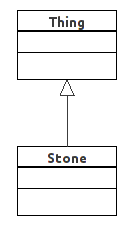
\includegraphics[width=0.5\linewidth]{property-types}}
    \end{minipage}
    \caption{Пример преобразования типов}
    \label{img:property-types}
\end{figure}
   

        \item В отображении отношений (Рис.~\ref{img:property-relations}) $F_R$ любому PDDL-предикату соответствует ассоциация UML либо атрибут UML-класса. Причем, если предикат \textit{унарный}, то он отображается в атрибут, иначе в ассоциацию; также разным предикатам соответствуют разные ассоциации/атрибуты:
    
        \begin{center}
        $\forall rel \in Relations_{PDDL} \Rightarrow F_R(rel) \in Relations_{UML} \cup Attributes_{UML}$;\\
        $\forall rel_1, rel_2 \in Relations_{PDDL}, rel_1 \neq rel_2 \Rightarrow F_R(rel_1) \neq F_R(rel_2)$; \\
        \end{center}

    
\begin{figure}[h]
    \hfill
    \begin{minipage}[h]{0.50\linewidth}
        {\raggedright
        \begin{verbatim}
    (:predicates
      (right ?phi - Philosopher 
          ?for - Fork)
      (hungry ?phi - Philosopher)
    )
        \end{verbatim} 
        }
    \end{minipage}
    \hfill
    $\rightarrow$
    \hfill
    \begin{minipage}[h]{0.45\linewidth}
        \center{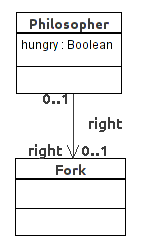
\includegraphics[width=0.5\linewidth]{property-relations}}
    \end{minipage}
    \caption{Пример преобразования отношений}
    \label{img:property-relations}
\end{figure}       


        \item 
        Введем вспомогательное отображение объектов в соответствующие типы $Type: o \in S \rightarrow Types$, отображение экземпляров отношений в соответствующие типы отношений $Relation: rel \in S \rightarrow Relations$, отображение экземпляров атрибутов в соответствующие атрибуты $Attribute_{UML}: atr \in S_{UML} \rightarrow Attributes_{UML}$, и отображение состояний $F_S: S_{PDDL} \rightarrow S_{UML}$,  для корректного определения которого потребуем выполнения следующих свойств:
       \begin{center}
        $\forall s = \{ o_1, ..., o_n, rel_1, ..., rel_m \} \in S_{PDDL} \Rightarrow$ \\ 
        $\Rightarrow F_S(s) = \{ o_1', ..., o_n', rel_1', ..., rel_k', atr_1, ..., atr_k \} \in S_{UML}$;  \\
                
        $\forall o_i \in s \Rightarrow F_T(Type_{PDDL}(o_i)) = Type_{UML}(o_i') $; \\  
        $\forall rel_i \in s \Rightarrow F_R(Relation_{PDDL}(rel_i)) = $
\[ = \left\{ 
    \begin{array}{l l}
        Attribute_{UML}(rel_k') & \quad \text{, $Relation_{PDDL}(rel_i)$~--- унарный предикат;} \\
        Relation_{UML}(atr_l) & \quad \text{, иначе;}
    \end{array}     
\right.\]
        \end{center}
        
        Тогда отображение задач (Рис.~\ref{img:property-tasks}) $F_C$ должно обладать следующим свойством корректности относительно отображения $F_S$ :
        
        \begin{center}
            $\forall t = \langle I, G \rangle \in T_{PDDL} \Rightarrow F_C(t) = \langle F_S(I), G' \rangle$; \\
            $\forall s \in S_{PDDL} \Rightarrow G(s) = True \Leftrightarrow G'(F_S(s)) = True $
        \end{center}
   
\begin{figure}[h]
    \center{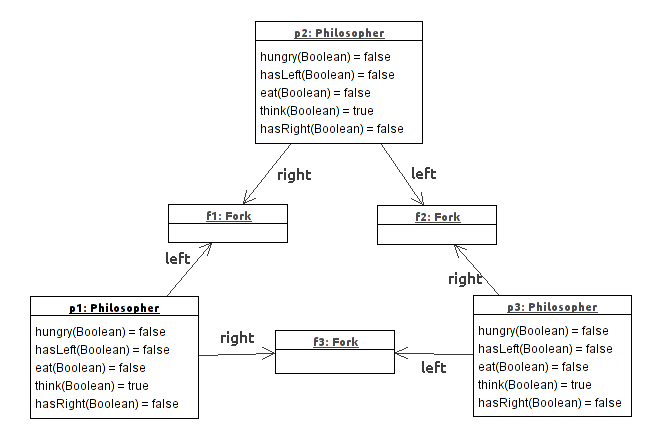
\includegraphics[width=1\linewidth]{property-tasks}}
    \caption{Пример преобразования состояний}
    \label{img:property-tasks}
\end{figure}   
           
        \item
    Отображение действий (Рис.~\ref{img:property-actions}) $F_A$ должно удовлетворять следующим требованиям:
    \begin{center}
        $\forall a \in Actions_{PDDL} \Rightarrow F_A(a) \in Actions_{UML}$; \\    
    
        $\forall a_1, a_2 \in Actions_{PDDL}, a_1 \neq a_2 \Rightarrow F_A(a_1) \neq F_A(a_2)$; \\        
 
        $\forall a \in Actions_{PDDL}, partypes_a = \langle c_1, c_2, ..., c_n \rangle \Rightarrow F_A(a) = a', partypes_{a'} = \langle F_T(c_1), F_T(c_2), ..., F_T(c_n)\rangle$; \\
 
        $\forall a \in Actions_{PDDL}, \forall s \in S_{PDDL}, a' = F_A(a) \Rightarrow precond_a(s, p) = True, p \subset s \Leftrightarrow precond_{a'}(F_S(s), p') = True, p' = F_S(p)$, и \\
        
        $effect_{a'}(F_S(s), p') = F_S(effect_a(s, p)), p \subset s, p' = F_S(p) $;
    \end{center}            
       
\begin{figure}[h]
    \begin{minipage}[h]{1\linewidth}
        \center{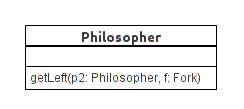
\includegraphics[width=0.5\linewidth]{property-actions}}    
    \end{minipage} \\
    \vfill
    {\centering $+$ \\ \medskip } 
        \begin{minipage}[h]{0.43\linewidth}
        
           \begin{verbatim}
    context Philosopher::getLeft(p2: Philosopher, f: Fork)
        pre 
            self.left = f 
            and p2.right = f 
            and self.hungry 
            and not p2.hold->includes(f)
        post
            self.hasLeft
            and self.hold = self.hold@pre->including(f)
            and not self.hungry
           \end{verbatim}
        \end{minipage}

    \begin{center}
        \begin{minipage}{0.8\linewidth}
            \caption{Один из вариантов преобразования действий с ограничениями на OCL на примере $getLeft$ }
        \end{minipage}    
    \end{center}

    \label{img:property-actions}
\end{figure}      

    \item
        Планом, решающим задачу $t = \langle I, G \rangle$ называется последовательность 
        \begin{center}
            $\langle s_1, a_1, p_1  \rangle, \langle s_2, a_2, p_2  \rangle, ..., \langle s_N, \emptyset, \emptyset \rangle \in Plans(t)$, \\ $s_i \in S, a_i \in Actions, p_i \subset s_i$
        \end{center}
        такая, что $s_1 = I, s_i = effect_{a_{i-1}}(s_{i-1}, p_{i-1}), i > 1$ и $G(s_N) = True$ где $Plans(t)$~--- множество планов, решающих задачу $t$.      
        
       
        Введем вспомогательное отображение планов $F_P: Plans_{PDDL}(t) \rightarrow Plans_{UML}(t)$:
            \begin{center}
                $\forall p = \langle s_1, a_1, p_1  \rangle, \langle s_2, a_2, p_2  \rangle, ..., \langle s_N, \emptyset, \emptyset  \rangle \in Plans_{PDDL}(t) \Rightarrow $\\
            $F_P(p) = \langle F_S(s_1), F_A(a_1), F_S(p_1)  \rangle, \langle F_S(s_2), F_A(a_2), F_S(p_2)  \rangle, ..., \langle F_S(s_N), \emptyset, \emptyset  \rangle \in Plans_{UML}(t) $  
            \end{center}
            
        Преобразование $F$ должно обладать свойством сохранения планов:
        
        \begin{center}
            $\forall t = \langle I, G\rangle \in T_{PDDL}, p \in Plans_{PDDL}(t) 
            \Leftrightarrow F_P(p) \in Plans_{UML}(t) $

        \end{center}
    \end{enumerate}
    
    
    Данное преобразование довольно легко формализовать и реализовать для PDDL-описаний, использующих только подмножество STRIPS. Какие возможности PDDL за пределами STRIPS может поддержать разрабатываемое средство, каким образом их представлять в UML-моделях ~--- это все еще является открытым вопросом и темой для исследований. Сложности могут возникнуть, например, в необходимости задания ограничений на целевое состояние с использованием кванторов, что невозможно сделать только лишь с помощью диаграмм объектов. Другой сложностью может быть трансляция длительных действий PDDL, например, во временные диаграммы UML. Существенной подзадачей является также преобразование предусловий и эффектов операций из PDDL в OCL. 
     
   
\section*{Существующие решения}
    
\subsection*{itSIMPLE}
    Одной из сред поддержки процессов, связанных с планированием, является среда itSIMPLE \cite{itsimple} (Integrated Tools Software Interface for Modeling PLanning Environments). В ней предложено использовать UML-модели со специальной семантикой некоторых элементов. Описанные модели можно автоматически транслировать на PDDL, а затем подать на вход планировщикам. Полученный план затем можно визуализировать внутри среды. Под визуализацией понимается отображение в виде диаграмм объектов последовательных состояний, через которые проходит система. Так или иначе, средство решает обратную задачу, а не задачу, поставленную в данной работе.
    
    На Рис. \ref{img:its_phil_domain} показано описание классов предметной области  "Обедающие философы". С помощью диаграмм состояний в itSIMPLE можно описать, в каких состояниях может находиться объект и как осуществляются переходы между ними. Описания переходов не совсем соответствуют спецификации UML, в частности, переходы показаны как методы с параметрами. Тем не менее у переходов существуют охранные условия (предусловия) и действия (эффекты), которые задаются на языке OCL. На Рис. \ref{img:its_phil_precond} и Рис. \ показаны диаграмма состояний и пример описания предусловий на OCL.
    
    \begin{figure}[h]
        \center{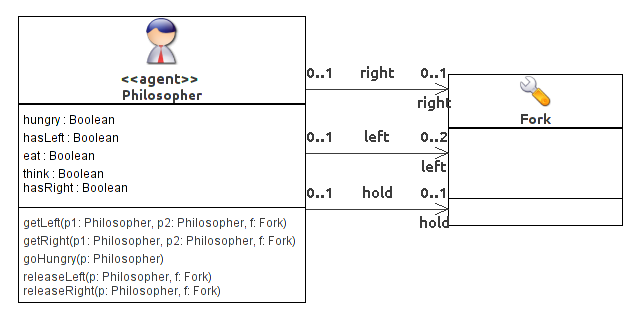
\includegraphics[width=1\linewidth]{its_phil_domain}}
        \caption{Пример описания классов предметной области в itSIMPLE}
        \label{img:its_phil_domain}

    \end{figure}
    
    \begin{figure}[h] 
        \center{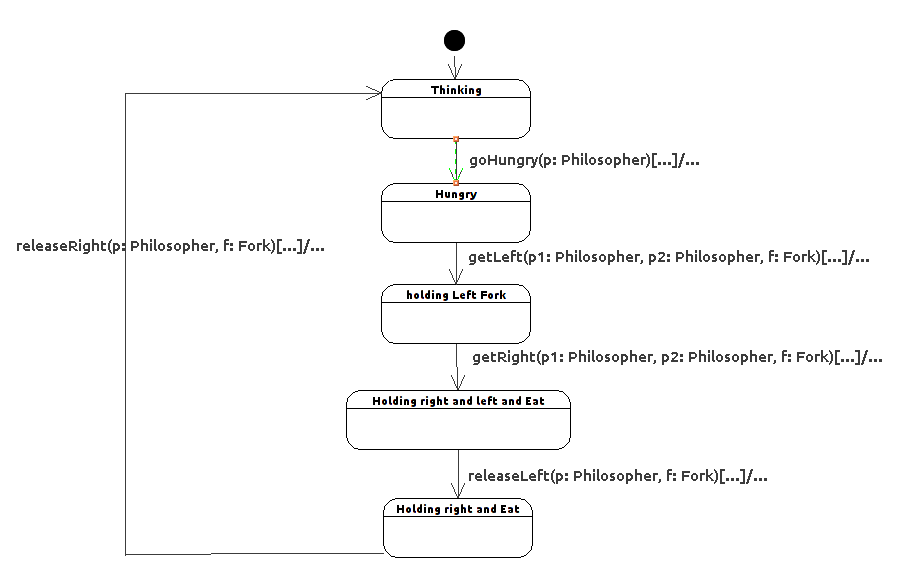
\includegraphics[width=1\linewidth]{its_phil_states}}
        \caption{Пример описания диаграммы состояний объектов в itSIMPLE}
        \label{img:its_phil_states}

    \end{figure}
    
    \begin{figure}[h] 
        \center{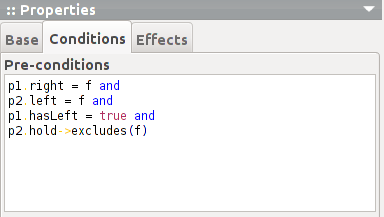
\includegraphics[width=0.5\linewidth]{its_phil_precond}}
        \caption{Пример описания действия \texttt{getRight} в itSIMPLE}
        \label{img:its_phil_precond}

    \end{figure}
        
    
\subsection*{MoDisco}
    Инструмент позволяет создавать модели различных систем, используя специальные Discoverer'ы, которые должны "исследовать" и обработать входные данные. На данный момент   Discoverer'ы существуют в основном только для Java-кода и JAR-архивы. Кроме того, MoDisco находится в стадии разработки и о скором создании PDDL-Discover'ов говорить не приходится. На  Рис. \ref{img:modisco_overview} показан общий вид работы средства.
    
    \begin{figure}[h]
        \center{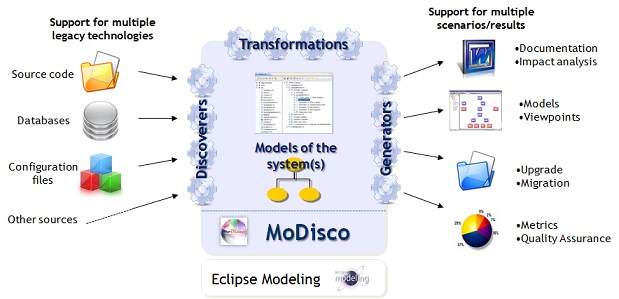
\includegraphics[width=1\linewidth]{modisco_overview}}
        \caption{Схема работы средства MoDisco}
        \label{img:modisco_overview}

    \end{figure}    

\subsection*{Решение задач инженерии знаний средствами объектно-ориентированной  инженерии программного обеспечения}    

В статье \cite{mal-manz} предлагается использовать стандартную нотацию UML и язык объектных ограничений OCL для описания предметных областей и задач планирования.

В рамках статьи было предложено задавать описания предметных областей в виде диаграмм классов UML, а пред- и постусловия~--- в виде ограничений на OCL, начальные условия~--- в виде диаграмм объектов, а цели~--- в виде выражений языка OCL. 

Также, был предложен способ перевода такой нотации в PDDL-описания для планировщика. А сам генератор был реализован на основе программного средства Acceleo, реализующего стандарт MOFM2T\cite{mofm2t}. 

    
\subsection*{Другие средства}
     Подавляющее большинство инструментов, реализующих преобразование каких-либо текстовых данных в UML-модели, существует для работы с языками программирования, как правило, объектно-ориентированными, а не с языками представления знаний. Поэтому, использование этих инструментов для решения поставленной задачи невозможно.  
    
    В далеком 2005 создавалось средство GIPO (Graphical Interface for Planning with Objects)\cite{gipo}~--- графический интерфейс для планирования с объектами. Среди его возможностей было: поддержка классического планирования, HTN (иерархические  сети задач), поддержка длительных действий, различные редакторы для создания описаний предметных областей и задач планирования, статический анализ и динамическое тестирование плана, встроенные и сторонние планировщики и трансляция в PDDL. К сожалению, там была предложена своя графическая нотация, не имеющая никакого отношения к UML. Ныне проект заброшен.   
    
\section*{Исследование и построение решения задачи}
   
    Готовых средств, решающих задачу, поставленную в данной дипломной работе, нет, поэтому оправданно создание собственного средства. 

    За основу разрабатываемой нотации на основе UML было решено взять нотацию, предложенную в статье \cite{mal-manz}, и, если необходимо, дополнить её новыми элементами UML или предложить новый способ представления элементов PDDL. 

    С поддержкой преобразования такого подмножества PDDL, как STRIPS, проблем возникнуть не должно. Вопрос поддержки возможностей PDDL за пределами STRIPS остается открытым в работе на данный момент. Существующие стандарты нуждаются в более детальном изучении.

    Существует средство PDDL4J, в котором заявлено, что реализуется парсер PDDL-описаний и предоставляется Java API для дальнейшего анализа. К сожалению, пока непонятно, какую версию PDDL поддерживает это средство. Это направлению нуждается в более детальной проработке.
     
    В случае, если PDDL4J нас не устроит (вопросы лицензии, обнаруженные ошибки и т.д.), то вести разработку предполагается опираясь на универсальные фреймворки для создания средств компиляции и анализа. Для создания парсера PDDL грамматики возможно использование ANTLR~\cite{antlr}. 
    
    

\newpage
\begin{thebibliography}{00}

\bibitem{norwig-ai}
\textbf{Рассел С., Норвиг П.} \textit{Искусственный интеллект: современный подход, 2-е изд.} М. : Вильямс, 2006. 1408 с.

\bibitem{strips}
\textbf{Fikes R., Nilsson N.} \textit{STRIPS: a new approach to the application of theorem
proving to problem solving // Artificial Intelligence}. 1971. 2. P. 189-208.

\bibitem{pddl3}
\textbf{Gerevini, A., Long, D.} \textit{Plan constraints and preferences in PDDL3.} Technical Report, Univ. Brescia, Italy, 2005. 12p.

\bibitem{rambo-uml2}
\textbf{Рамбо Дж., Блаха М.} \textit{UML 2.0. Объектно-ориентированное моделирование и разработка, 2-е изд.} СПб. : Питер, 2007

\bibitem{icaps-1}
\textbf{Vaquero T.S., Silva J.R., Beck J.C.} A Brief Review of Tools and Methods for Knowledge Engineering for Planning and Scheduling. // Proceedings of the Knowledge Engineering for Planning and Scheduling (KEPS) workshop. The 21th International Conference on Automated Planning and Scheduling (ICAPS 2011). Freiburg. Germany. 2011

\bibitem{icaps-2}
\textbf{Vaquero T.S., Costa C., Tonidandel F., Igreja H., Silva J.R., Beck J.C.} Planning and Scheduling Ship Operations on Petroleum Ports and Platforms. // Proceedings of the ICAPS 2012 Workshop on Scheduling and Planning Applications (SPARK). 2012. pp. 8-16.

\bibitem{use}
\textbf{Gogolla M., Büttner F., Richter M.}. \textit{USE: A UML-Based Specification Environment for Validating UML and OCL.} Science of Computer Programming, 69:27-34, 2007.

\bibitem{gipo}
Graphical Interface for Planning with Objects. GIPO project. \textit{(http://planform.hud.ac.uk/gipo/gipo\_home.html)} 

\bibitem{mal-manz}
\textbf{Малышко В. В., Манжосов А. Н.} Решение задач инженерии знаний средствами объектно-ориентированной инженерии программного обеспечения. // Программные системы и инструменты. Тематический сборник No 13. М.: Изд-во факультета ВМиК МГУ, 2012. С. 44-54.


\bibitem{ocl}
\textbf{Warmer, Kleppe.} \textit{The Object Constraint Language: Getting Your Models Ready for MDA, Second Edition.} Addison-Wesley, 2003.

\bibitem{itsimple}
\textbf{Vaquero T. S., Tonaco R. et al.} \textit{itSIMPLE4.0: Enhancing the Modeling
Experience of Planning Problems.} Proceedings of the ICAPS 2012 System
Demonstration, São Paulo : s.n., 2012. pp. 11-14.

\bibitem{mofm2t}
Object Management Group MOF Model to Text Transformation Language, v 1.0 2008 \textit{(http://www.omg.org/spec/MOFM2T/1.0/PDF)}

\bibitem{antlr}
\textbf{Terence Parr.} \textit{ The Definitive ANTLR 4 Reference}, 2013. 328p.





\end{thebibliography}

\end{document}          
